\documentclass[conference]{IEEEtran}
\usepackage[utf8]{inputenc}
\usepackage[spanish,es-nodecimaldot]{babel}
\usepackage{amsmath,amssymb,amsfonts}
\usepackage{algorithmic}
\usepackage{graphicx}
\usepackage{textcomp}
\usepackage{xcolor}
\usepackage{hyperref}
\usepackage{booktabs}
\usepackage{listings}
\usepackage{microtype}
\usepackage{tabularx}
\usepackage{cite}

% Configuración de listados de código fuente
\definecolor{codegreen}{rgb}{0,0.6,0}
\definecolor{codegray}{rgb}{0.5,0.5,0.5}
\definecolor{codepurple}{rgb}{0.58,0,0.82}
\definecolor{backcolour}{rgb}{0.96,0.96,0.96}

\lstdefinestyle{estilocodigo}{
    backgroundcolor=\color{backcolour},   
    commentstyle=\color{codegreen},
    keywordstyle=\color{magenta},
    numberstyle=\tiny\color{codegray},
    stringstyle=\color{codepurple},
    basicstyle=\ttfamily\footnotesize,
    breakatwhitespace=false,         
    breaklines=true,                 
    captionpos=b,                    
    keepspaces=true,                 
    numbers=left,                    
    numbersep=5pt,                  
    showspaces=false,                
    showstringspaces=false,
    showtabs=false,                  
    tabsize=2
}
\lstset{style=estilocodigo}

\begin{document}

% =========================================================================
% ENCABEZADO Y METADATOS DEL DOCUMENTO (EDITAR AQUÍ)
% =========================================================================
\title{Diseño e Implementación de una Plataforma Web Editorial Multicanal Basada en el Patrón Arquitectónico Modelo-Vista-Controlador (MVC)\\
{\footnotesize \textsuperscript{*}Proyecto de Cátedra -- Hackathon de Arquitectura de Sistemas}}

\author{
    \IEEEauthorblockN{Marcos Josué García Maldonado}
    \IEEEauthorblockA{\textit{Facultad de Ingeniería} \\
    \textit{Universidad Mesoamericana}\\
    Carné: 202408055 \\
    marcosjgm@umes.edu.gt}
    \and
    \IEEEauthorblockN{Arturo Alejandro Maldonado Orozco}
    \IEEEauthorblockA{\textit{Facultad de Ingeniería} \\
    \textit{Universidad Mesoamericana}\\
    Carné: 2023080110 \\
    20arturomaldonado@umes.edu.gt}
    \and
    \IEEEauthorblockN{Sebastián Rodrigo Rodas Pineda}
    \IEEEauthorblockA{\textit{Facultad de Ingeniería} \\
    \textit{Universidad Mesoamericana}\\
    Carné: 202408060 \\
    srodas477@umes.edu.gt}
}

\maketitle

% =========================================================================
% RESUMEN (ABSTRACT) Y PALABRAS CLAVE
% =========================================================================
\begin{abstract}
El presente artículo expone el diseño, desarrollo e implementación técnica de una Plataforma Web Editorial Multicanal concebida bajo el marco de la Hackathon de Arquitectura de Sistemas. El sistema atiende la complejidad operativa de la industria editorial contemporánea mediante la unificación de canales de venta minorista y transacciones corporativas B2B. La arquitectura adoptada se cimenta en la aplicación rigurosa del patrón arquitectónico Modelo-Vista-Controlador (MVC), asegurando una separación estricta entre la capa de presentación, la orquestación de servicios y el dominio de negocio. Se integró un motor matemático de descuentos dinámicos ejecutado exclusivamente en la capa del Modelo, un esquema de seguridad basado en roles (RBAC) con cinco perfiles de acceso, un protocolo de idempotencia criptográfica dual (RAM y PostgreSQL) mediante firmas HMAC-SHA256, un limitador temporal de checkout de 10 minutos con sincronización reactiva vía WebSockets (Socket.IO), y almacenamiento en la nube de recursos multimedia con Cloudinary. La solución garantiza alta disponibilidad, mantenibilidad, modularidad y apego a las directrices de integridad transaccional ACID.
\end{abstract}

\begin{IEEEkeywords}
Modelo-Vista-Controlador (MVC), Arquitectura de Software, Idempotencia Criptográfica, WebSockets, Control de Acceso Basado en Roles (RBAC), PostgreSQL, Node.js.
\end{IEEEkeywords}

% =========================================================================
% I. INTRODUCCIÓN
% =========================================================================
\section{Introducción}
\IEEEPARstart{L}{a} transformación digital de la industria editorial demanda ecosistemas de software con alta capacidad de adaptación para gestionar inventarios bibliográficos distribuidos, modelos de precios heterogéneos y mecanismos de venta que abarcan tanto al consumidor individual como a clientes institucionales (universidades, colegios y redes de bibliotecas). La problemática central radica en que los sistemas de comercio electrónico convencionales suelen acoplar indebidamente la lógica de cálculo financiero con los controladores HTTP o las plantillas de vista, derivando en arquitecturas monolíticas frágiles, de difícil depuración y propensas a inconsistencias en auditorías contables.

Ante este desafío, la Hackathon de Arquitectura de Sistemas plantea el desarrollo de una plataforma web integral cuya premisa irremplazable es el cumplimiento estricto del patrón arquitectónico Modelo-Vista-Controlador (MVC). En este marco, el sistema no solo debe solventar la navegación de catálogo y el carrito de compras, sino gobernar un flujo de cotizaciones comerciales B2B, aplicar matrices dinámicas de descuento acumulativo, prevenir la duplicidad transaccional en ambientes de alta concurrencia mediante idempotencia garantizada, y limitar la persistencia temporal de sesiones de compra a un horizonte no mayor a 10 minutos con retroalimentación en tiempo real.

El presente artículo documenta la arquitectura global del sistema, desglosando la estructura de entidades de datos, la encapsulación matemática en los modelos, el esquema de autorización y los mecanismos de comunicación bidireccional implementados.

% =========================================================================
% II. ARQUITECTURA DE SOFTWARE (PATRÓN MVC)
% =========================================================================
\section{Arquitectura del Sistema (Patrón MVC)}

\subsection{Separación Estricta de Responsabilidades}
Para salvaguardar los principios de alta cohesión y bajo acoplamiento, la plataforma se estructura en tres capas conceptualmente aisladas:

\begin{enumerate}
    \item \textbf{Capa Modelo (Model):} Constituye el núcleo de la aplicación. Alberga las definiciones de entidad, el esquema relacional mapeado a través del ORM Sequelize, las restricciones de integridad y, primordialmente, las reglas dinámicas de negocio. Siguiendo las directrices del proyecto, queda terminantemente prohibida la inclusión de elementos de interfaz gráfica (HTML), manipulación directa del protocolo HTTP o delegación de cálculos contables a capas externas.
    \item \textbf{Capa Controlador (Controller):} Actúa como director y orquestador. Captura las solicitudes entrantes (HTTP/REST y eventos WebSocket), delega la ejecución de operaciones analíticas o transaccionales a los Modelos pertinentes, y emite respuestas en formatos estructurados estándar (JSON). No contiene sentencias SQL manuales ni lógica de liquidación financiera.
    \item \textbf{Capa Vista (View):} Responsable exclusiva de la presentación y experiencia de usuario. Opera de forma completamente desacoplada de la base de datos, consumiendo únicamente los datos entregados por los controladores para renderizar interfaces responsivas.
\end{enumerate}

\subsection{Topología Arquitectónica}
La Fig.~\ref{fig:arquitectura} ilustra el flujo de comunicación y el desacoplamiento entre las capas de la plataforma:

\begin{figure}[htbp]
\centering
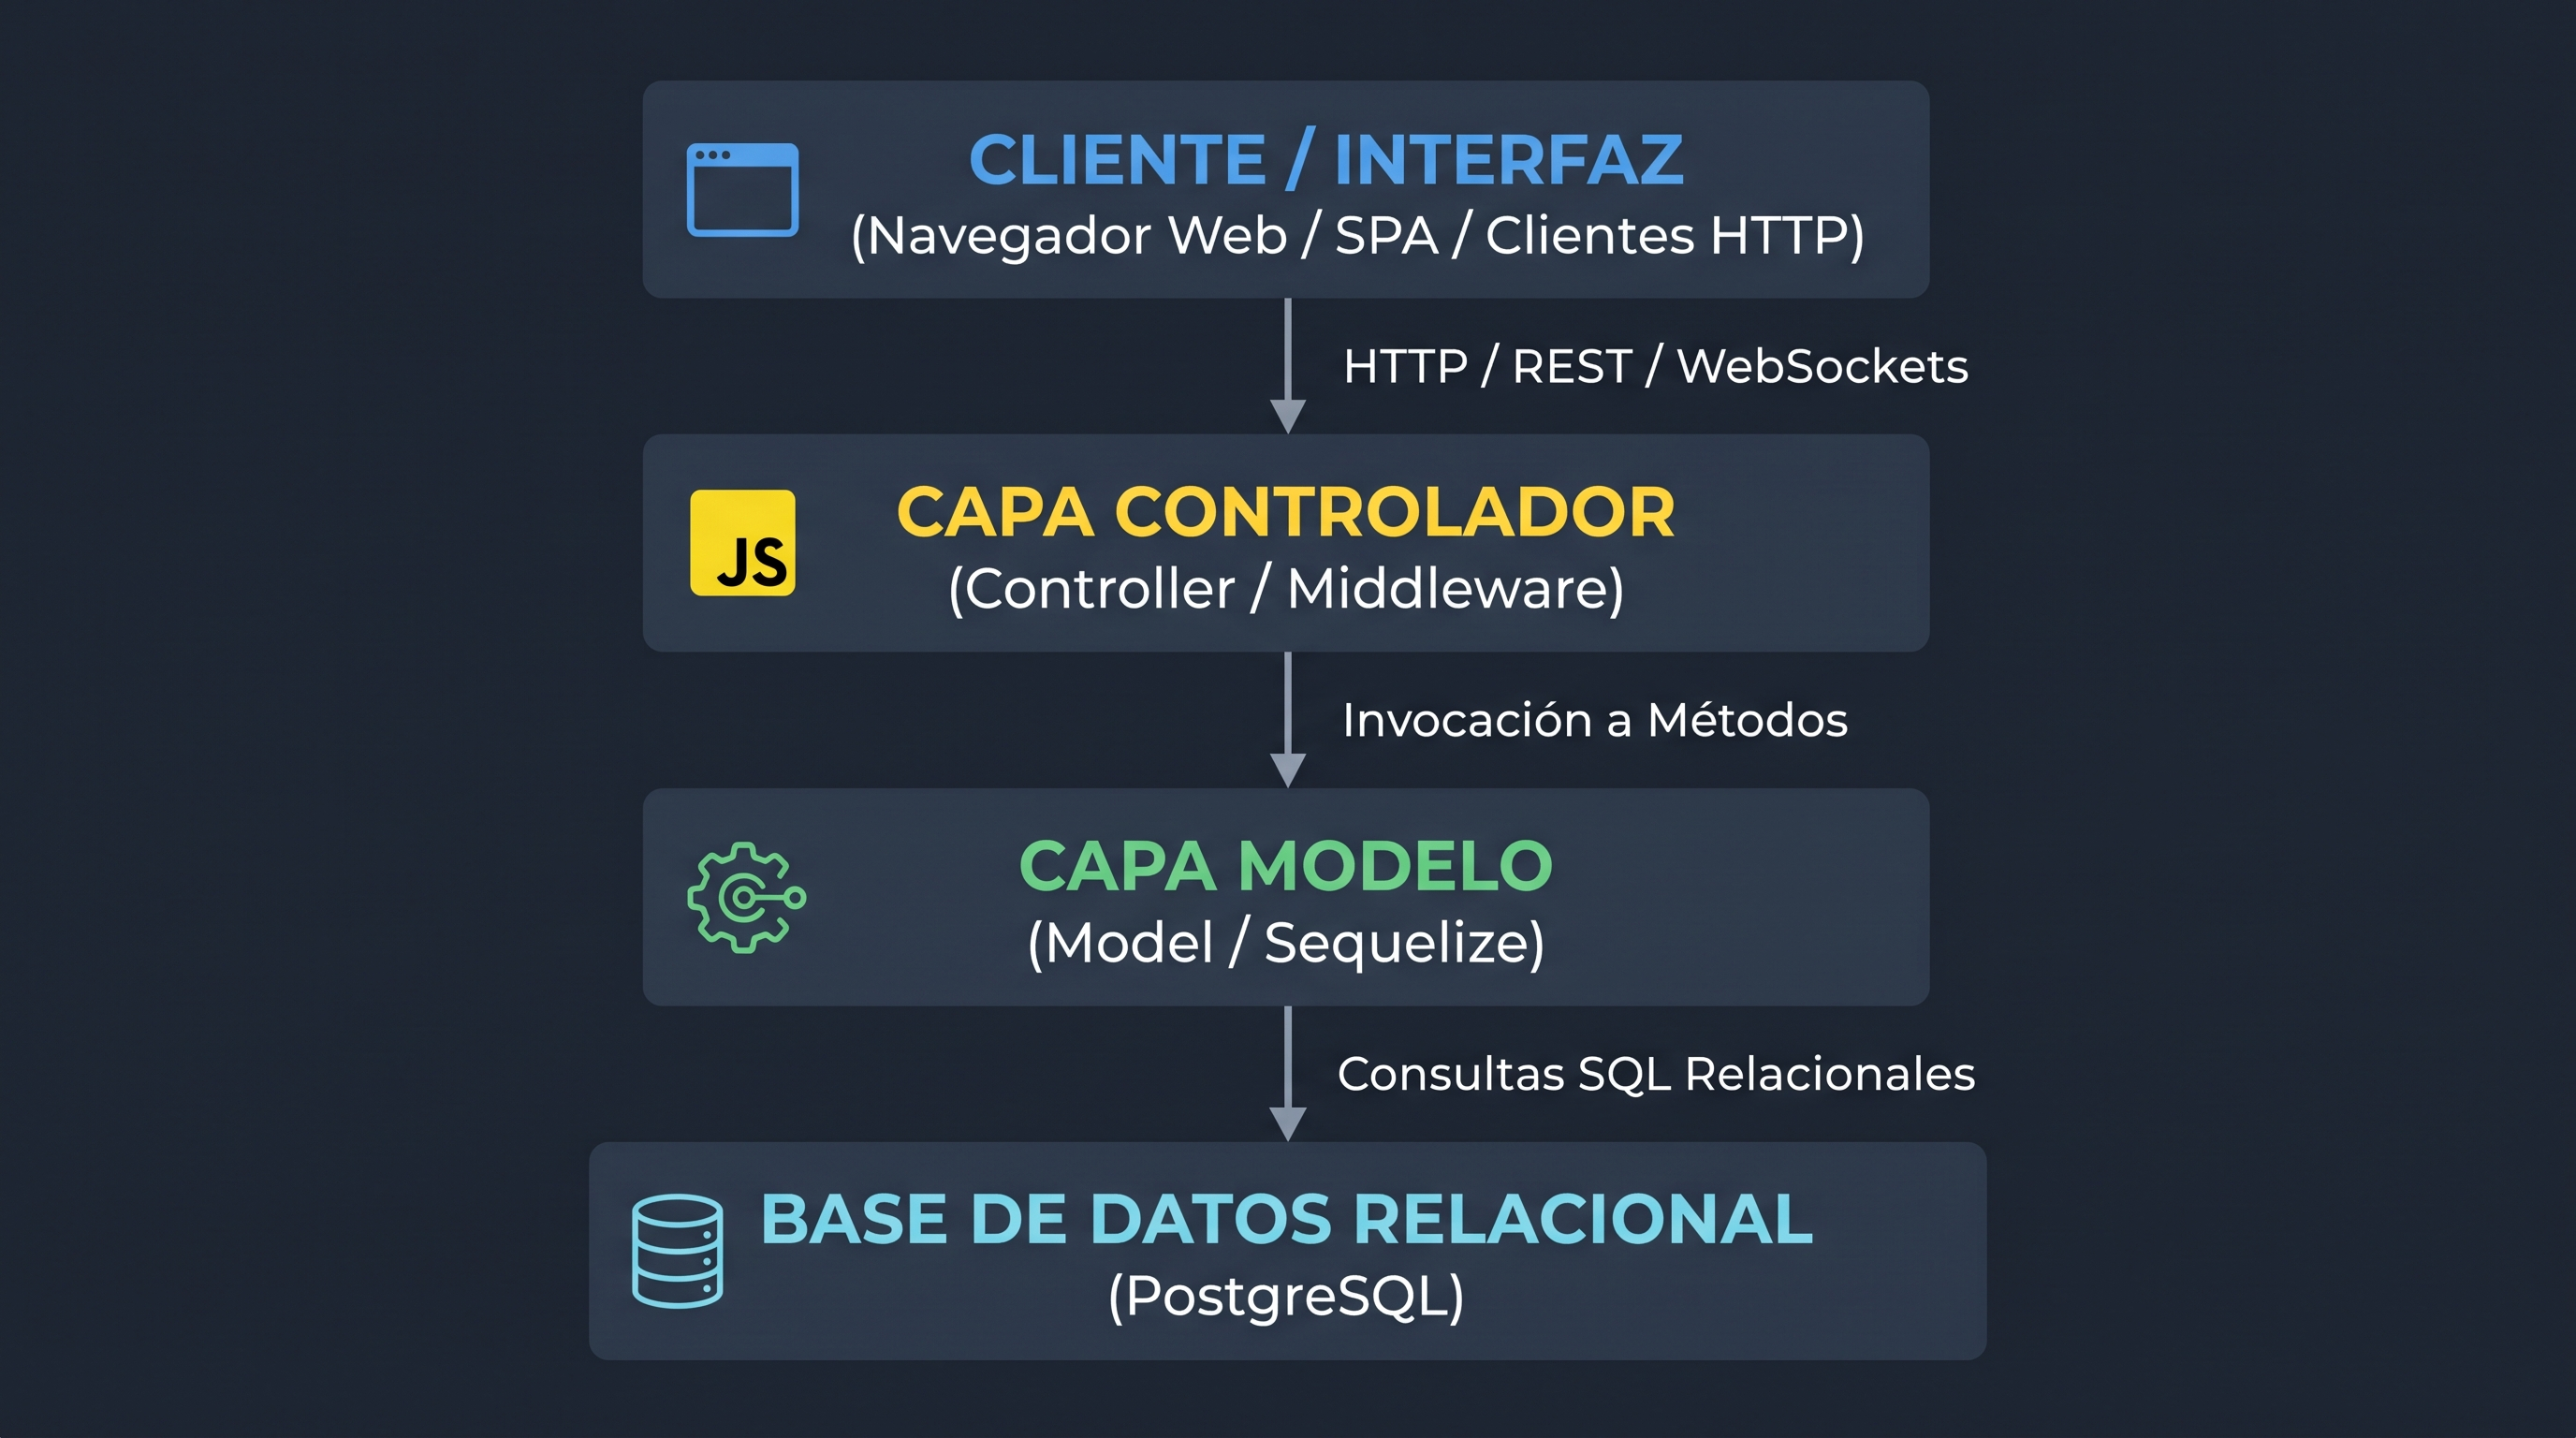
\includegraphics[width=\columnwidth]{TopologiaArquitectonica.jpeg}
\caption{Topología y Arquitectura Multicapa del Sistema Editorial.}
\label{fig:arquitectura}
\end{figure}

% =========================================================================
% III. DISEÑO Y MODELO DE BASE DE DATOS
% =========================================================================
\section{Diseño y Modelo de Base de Datos}
La persistencia de la información descansa sobre el motor relacional PostgreSQL (v14+). El esquema está compuesto por 18 tablas normalizadas en Tercera Forma Normal (3FN), garantizando integridad referencial mediante claves foráneas con políticas de actualización y eliminación en cascada controladas.

\subsection{Entidades Fundamentales}
\begin{itemize}
    \item \textbf{Gestión Bibliográfica:} Estructurada mediante las tablas \texttt{libros}, \texttt{autores}, \texttt{editoriales}, \texttt{generos} y \texttt{formatos}. Se implementan tablas asociativas N:M (\texttt{libros\_autores}, \texttt{libros\_editoriales}, \texttt{libros\_generos}) para representar la multiplicidad de participantes en una obra.
    \item \textbf{Catálogo y Variantes:} La tabla \texttt{catalogo\_productos} vincula el libro con su formato físico o digital (Tapa Blanda, Tapa Dura, E-Book, Audiolibro), gestionando el ISBN, precio base y el stock disponible para despacho.
    \item \textbf{Seguridad y Usuarios:} Conectada mediante \texttt{usuarios}, \texttt{roles} y \texttt{perfiles\_institucionales}. Esta última almacena datos tributarios y de acreditación corporativa (NIT, razón social y sector de actividad).
    \item \textbf{Ventas y Transacciones:} Conformada por \texttt{carritos}, \texttt{carrito\_items}, \texttt{ordenes}, \texttt{orden\_detalles}, \texttt{checkout\_sesiones} e \texttt{idempotencias}.
    \item \textbf{Cotizaciones Comerciales B2B:} Modelada a través de \texttt{cotizaciones\_solicitudes} y \texttt{cotizaciones\_propuestas}, soportando el ciclo de negociación entre el cliente institucional y el asesor de ventas.
\end{itemize}

% =========================================================================
% IV. LÓGICA DE NEGOCIO Y MOTOR DE DESCUENTOS (RF-03.2)
% =========================================================================
\section{Lógica de Negocio y Motor de Descuentos}
En estricto apego al requerimiento funcional RF-03.2, la lógica de cálculo financiero fue encapsulada en el método estático \texttt{Carritos.calcularTotales} del Modelo, eliminando cualquier procesamiento contable en los controladores.

\subsection{Matriz de Reglas Dinámicas}
La formulación matemática de la liquidación opera según las siguientes ecuaciones:

\begin{equation}
S_{\text{base}} = \sum_{i=1}^{n} (P_{i} \times Q_{i})
\end{equation}
donde $P_i$ representa el precio base unitario y $Q_i$ la cantidad demandada del ítem $i$. El descuento por volumen de compra ($D_{\text{vol}}$) se asigna escalonadamente en función del volumen total $U = \sum Q_i$:

\begin{equation}
\%_{\text{vol}} = 
\begin{cases} 
0\%, & \text{si } 1 \le U \le 5 \\
5\%, & \text{si } 6 \le U \le 20 \\
10\%, & \text{si } 21 \le U \le 50 \\
15\%, & \text{si } U > 50 
\end{cases}
\end{equation}

\begin{equation}
D_{\text{vol}} = S_{\text{base}} \times \%_{\text{vol}}
\end{equation}

El subtotal resultante tras la aplicación del volumen ($S_{\text{vol}}$) sirve de base para el descuento institucional acumulativo ($D_{\text{inst}}$), exclusivo para entidades educativas o comerciales acreditadas:

\begin{equation}
S_{\text{vol}} = S_{\text{base}} - D_{\text{vol}}
\end{equation}

\begin{equation}
D_{\text{inst}} = 
\begin{cases} 
S_{\text{vol}} \times 0.08, & \text{si Rol} = \text{Institucional} \\
0, & \text{si Rol} \neq \text{Institucional}
\end{cases}
\end{equation}

Finalmente, el descuento global ($D_{\text{total}}$), la base imponible neta ($S_{\text{neto}}$), el Impuesto al Valor Agregado ($IVA$, 12\%) y el valor de liquidación definitivo ($T_{\text{final}}$) se obtienen según:

\begin{equation}
D_{\text{total}} = D_{\text{vol}} + D_{\text{inst}}
\end{equation}
\begin{equation}
S_{\text{neto}} = S_{\text{base}} - D_{\text{total}}
\end{equation}
\begin{equation}
IVA = S_{\text{neto}} \times 0.12
\end{equation}
\begin{equation}
T_{\text{final}} = S_{\text{neto}} + IVA
\end{equation}

La Tabla~\ref{tab:descuentos} resume los escenarios de prueba ejecutados para corroborar la precisión de la lógica en el Modelo.

\begin{table}[htbp]
\caption{Matriz de Liquidación y Descuentos Dinámicos}
\label{tab:descuentos}
\centering
\setlength{\tabcolsep}{3pt}
\resizebox{\columnwidth}{!}{%
\begin{tabular}{lcccc}
\toprule
\textbf{Escenario} & \textbf{Unidades} & \textbf{\% Vol.} & \textbf{\% Inst.} & \textbf{Total Final (Q)} \\
\midrule
Minorista Individual & 2  & 0\%  & 0\%        & Base + IVA \\
Minorista Mediano    & 10 & 5\%  & 0\%        & Base - 5\% + IVA \\
Institucional Básico & 4  & 0\%  & 8\%        & Base - 8\% + IVA \\
Institucional Medio  & 15 & 5\%  & 8\% acum.  & Descuento Mixto \\
Institucional Masivo & 60 & 15\% & 8\% acum.  & Beneficio Máximo \\
\bottomrule
\end{tabular}%
}
\vspace{1ex}
\end{table}

% =========================================================================
% V. SEGURIDAD, RBAC Y CONTROL DE ACCESO
% =========================================================================
\section{Seguridad y Control de Acceso (RBAC)}
El sistema implementa un modelo de Control de Acceso Basado en Roles (RBAC) granular que clasifica a los intervinientes en cinco categorías claramente tipificadas:

\begin{enumerate}
    \item \textbf{Visitante (Anónimo):} Consulta abierta de catálogo, landing y fichas técnicas. No puede operar carritos ni iniciar compras.
    \item \textbf{Cliente Minorista:} Compras a nivel individual, gestión de carrito propio e historial de órdenes personales.
    \item \textbf{Cliente Institucional:} Acceso a la matriz de precios corporativos (+8\% acumulativo) y emisión de solicitudes de pedidos especiales no disponibles en catálogo común.
    \item \textbf{Asesor de Ventas:} Acceso a la bandeja de cotizaciones, capacidad de asignar expedientes, formulación de propuestas económicas y seguimiento comercial.
    \item \textbf{Administrador:} Gobernanza completa del sistema, mantenimiento de libros y autores, ajuste de inventario, auditoría global y validación institucional.
\end{enumerate}

Las credenciales de acceso se protegen mediante la función de dispersión unidireccional Bcrypt con un factor de trabajo (\textit{salt rounds}) de 10. La autorización de endpoints se rige por tokens JSON Web Token (JWT) con separación de Access Token (vida útil corta) y Refresh Token.

% =========================================================================
% VI. MECANISMOS AVANZADOS: IDEMPOTENCIA Y TEMPORIZADOR
% =========================================================================
\section{Idempotencia y Checkout en Tiempo Real}

\subsection{Idempotencia Criptográfica Dual}
Para prevenir problemas de doble cobro o deducción duplicada de inventario ante pérdidas de paquetes o reintentos del usuario, el sistema incorpora un esquema de idempotencia soportado en la variable de entorno \texttt{IDEMPOTENCY\_KEY}. La llave de idempotencia se construye mediante HMAC-SHA256:

\begin{equation}
K_{\text{idemp}} = \text{HMAC-SHA256}(\text{Key}_{\text{env}}, \text{Payload}_{\text{tx}})
\end{equation}

El mecanismo opera en dos capas concurrentes:
\begin{itemize}
    \item \textbf{Capa en Memoria RAM:} Resuelve colisiones en milisegundos para peticiones concurrentes simultáneas.
    \item \textbf{Persistencia en BD (\texttt{idempotencias}):} Almacena la llave (\texttt{VARCHAR(255)}) junto con el payload de respuesta en formato \texttt{JSONB}. Si el servicio se reinicia, la solicitud retransmitida es reconocida y despachada con la cabecera \texttt{X-Idempotency-Replay: true} sin reinvocar la transacción en la base de datos.
    \item \textbf{Restricción Unívoca:} El campo \texttt{ordenes.idempotency\_key} posee un constraint \texttt{UNIQUE} que blinda la consistencia a nivel de motor SQL.
\end{itemize}

\subsection{Sesiones de Checkout de 10 Minutos y WebSockets}
El proceso de checkout establece una reserva temporal de inventario sujeta a una vigencia estricta de 600 segundos (10 minutos):
\begin{enumerate}
    \item Al iniciar el checkout (\texttt{POST /api/ordenes/iniciar-checkout}), se persiste un registro en la tabla \texttt{checkout\_sesiones} con los ítems y desgloses en \texttt{JSONB}, fijando la marca temporal \texttt{expira\_en}.
    \item El servidor activa un temporizador Socket.IO que transmite cada segundo el evento \texttt{checkout:tick} a la sala del usuario (\texttt{checkout:\{userId\}}).
    \item En caso de sobrepasar los 10 minutos sin confirmar la orden, el estado muta a \texttt{expirada}, se emite \texttt{checkout:expirado} y la API responde con código \texttt{410 Gone}, redireccionando forzosamente a la tienda.
    \item Si el usuario confirma en tiempo, la orden se crea dentro de una transacción atómica gestionada por Sequelize (\texttt{transaction.commit()}), la sesión pasa a \texttt{completada} y se emite \texttt{reporte:nueva\_venta} a los paneles de administración en tiempo real.
\end{enumerate}

% =========================================================================
% VII. INTEGRACIONES EXTERNAS Y DOCUMENTACIÓN
% =========================================================================
\section{Integraciones Externas y Documentación}

\subsection{Almacenamiento Multimedia con Cloudinary}
Para el almacenamiento de portadas de libros requeridas en el catálogo (\texttt{models/Libros.js}), se implementó una integración en la nube con Cloudinary respaldada por un middleware de procesamiento en memoria con Multer. La API permite tanto la subida directa de archivos binarios (\texttt{multipart/form-data}) como la asignación de URLs preexistentes, alojando las imágenes de forma optimizada mediante CDN global.

\subsection{Documentación Interactiva Swagger / OpenAPI 3.0}
Todos los endpoints desarrollados se documentaron rigurosamente bajo el estándar OpenAPI 3.0 mediante Swagger UI. La interfaz interactiva se encuentra disponible en las rutas \texttt{/api-docs} y \texttt{/docs}, permitiendo la prueba autenticada de rutas mediante inyección de Bearer Tokens y encabezados de idempotencia.

% =========================================================================
% VIII. METODOLOGÍA, PRUEBAS Y RESULTADOS
% =========================================================================
\section{Metodología de Desarrollo y Pruebas}
El desarrollo del proyecto se condujo bajo la metodología ágil Scrum adaptada a hackathon, apoyada en un estricto control de versiones con Git mediante ramas funcionales (\textit{feature branches}) unificadas sobre la rama principal \texttt{Dev}.

Se elaboraron baterías de pruebas de integración para validar:
\begin{itemize}
    \item Consistencia de cálculo en el motor de descuentos ante carritos mixtos de 1 a 100 ejemplares.
    \item Resistencia a ataques de inyección SQL mediante sentencias parametrizadas del ORM.
    \item Verificación de caducidad temporal a los 600 segundos exactos en sesiones de checkout.
    \item Comportamiento idempotente ante ráfagas de 5 peticiones simultáneas con idéntico identificador.
\end{itemize}

Los resultados confirmaron tiempos de respuesta promedio inferiores a 120 ms en consultas locales y total integridad referencial en las 18 tablas relacionales.

% =========================================================================
% IX. CONCLUSIONES
% =========================================================================
\section{Conclusiones}
La aplicación sistemática del patrón arquitectónico Modelo-Vista-Controlador (MVC) posibilitó la creación de una plataforma editorial sólida, escalable y mantenible. Se demostró que la delegación exclusiva de las reglas financieras a la capa del Modelo protege la lógica de dominio ante cambios en la infraestructura de transporte o presentación. La combinación de transacciones ACID en PostgreSQL, doble persistencia de idempotencia (HMAC-SHA256) y sincronización reactiva bidireccional mediante WebSockets garantiza un flujo de ventas robusto, capaz de soportar operaciones masivas sin riesgo de sobreventa de inventario ni transacciones duplicadas.

% =========================================================================
% REFERENCIAS BIBLIOGRÁFICAS (FORMATO IEEE)
% =========================================================================
\begin{thebibliography}{00}

\bibitem{gamma1994}
E. Gamma, R. Helm, R. Johnson, y J. Vlissides, \textit{Design Patterns: Elements of Reusable Object-Oriented Software}. Boston, MA, USA: Addison-Wesley, 1994.

\bibitem{fowler2002}
M. Fowler, \textit{Patterns of Enterprise Application Architecture}. Boston, MA, USA: Addison-Wesley, 2002.

\bibitem{martin2017}
R. C. Martin, \textit{Clean Architecture: A Craftsman's Guide to Software Structure and Design}. Boston, MA, USA: Prentice Hall, 2017.

\bibitem{ieee730}
\textit{IEEE Standard for Software Quality Assurance Processes}, IEEE Std 730-2014, 2014.

\bibitem{rfc7519}
M. Jones, J. Bradley, y N. Sakimura, ``JSON Web Token (JWT)'', RFC 7519, Internet Engineering Task Force (IETF), Mayo 2015.

\bibitem{rfc6455}
I. Fette y A. Melnikov, ``The WebSocket Protocol'', RFC 6455, Internet Engineering Task Force (IETF), Diciembre 2011.

\bibitem{postel1981}
J. Postel, ``Transmission Control Protocol'', RFC 793, Internet Engineering Task Force (IETF), Septiembre 1981.

\end{thebibliography}

\end{document}
